% \subsection{Data Loading and Inspection}
% The analysis began by loading the separate VIIRS (Visible Infrared Imaging Radiometer Suite) fire detection files for Algeria (\texttt{df\_fire\_dza}) and Tunisia (\texttt{df\_fire\_tun}).

% \begin{itemize}
%     \item \textbf{Initial Check:} Descriptive statistics \texttt{(describe())} were computed to understand the distribution, range, and central tendencies of numerical features like \texttt{frp} and brightness temperatures.
%     \item \textbf{Data Quality:} Inspection of data types, memory usage, and the percentage of missing values (\texttt{isnull().mean()}) confirmed data integrity and structure consistency across both datasets.
%     \item \textbf{Data Integration:} The two datasets were merged into a single GeoDataFrame, \texttt{df\_fire}, using the \texttt{pd.concat()} function, ready for combined regional analysis.
% \end{itemize}
\subsection{Data Loading and Inspection}

The analysis began by loading the datasets for Algeria (\texttt{df\_fire\_dza}) and Tunisia (\texttt{df\_fire\_tun}). An initial exploratory inspection was performed using descriptive statistics to assess the distribution and range of key numerical variables, including fire radiative power (\texttt{frp}) and brightness temperatures. Data quality was verified by examining data types, memory usage, and the proportion of missing values, confirming structural consistency and integrity across both datasets. Finally, the two datasets were merged using \texttt{pd.concat()} into a single GeoDataFrame (\texttt{df\_fire}), enabling unified regional analysis.


\subsection{Exploratory Data Analysis (EDA) and Visualization}

\begin{figure}[H]
    \centering
    
\includegraphics[width=0.45\textwidth]{\detokenize{images/Fire/frp values in map.png}}
    \caption{Geospatial distribution of fire events across Algeria and Tunisia. Points are colored by Fire Radiative Power (FRP), highlighting areas of highest fire intensity.}\label{fig:fire_spatial_map}
\end{figure}

The geospatial distribution of fire events was visualized using a scatter plot of \texttt{longitude} vs.\ \texttt{latitude}, with the color intensity mapped to \texttt{frp}. This visualization is essential for identifying fire clusters and high-intensity regions across the combined study area.
As shown in the map, the majority of fire points are concentrated in the northern regions, reflecting higher vegetation density and more favorable climatic conditions for fire occurrence compared to the arid southern areas


% \begin{figure} [H]
%     \centering
%     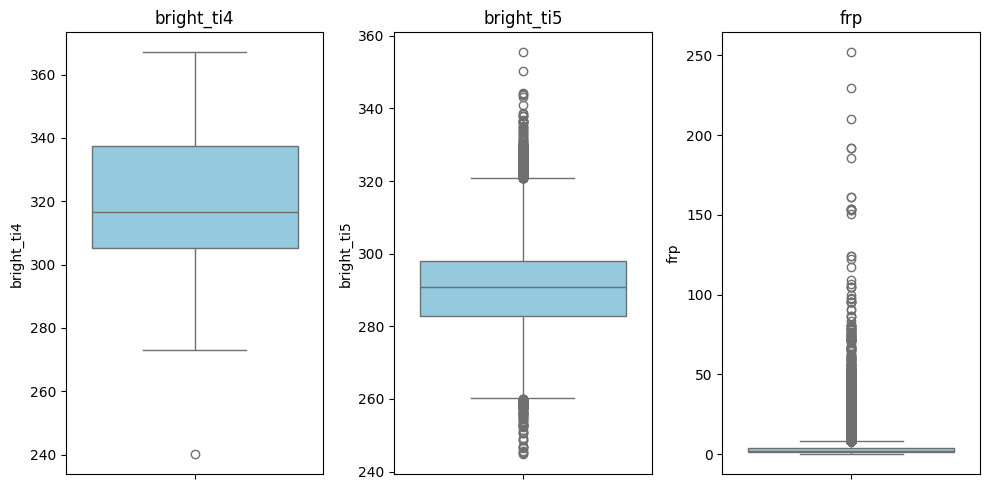
\includegraphics[width=0.8\textwidth]{images/Fire/boxplots.png}
%     \caption{Boxplots displaying the distribution of fire intensity metrics (\texttt{bright\_ti4, bright\_ti5, frp}), clearly illustrating the presence of extreme outliers (high-power fires) above the main interquartile range.}
%     \label{fig:boxplots}
% \end{figure}

% Boxplots (Figure \ref{fig:boxplots}) further confirmed the presence of significant outliers in the fire intensity metric $\texttt{bright\_ti5}$ and $\texttt{frp}$), due to the presence of extremely hot and large fire events.

